\documentclass[12pt,a4paper]{article}
\usepackage[margin=1in]{geometry}
\usepackage{graphicx,booktabs,hyperref,enumitem,xcolor,listings,float,amsmath,tikz}
\usepackage[utf8]{inputenc}
\usepackage{fancyhdr,titlesec}

\definecolor{primary}{HTML}{00D4AA}
\definecolor{darkbg}{HTML}{1A1A2E}
\hypersetup{colorlinks=true,linkcolor=darkbg,urlcolor=primary,citecolor=darkbg}

\pagestyle{fancy}
\fancyhf{}
\fancyhead[L]{\small\textcolor{gray}{Estate Agent AI — Project Report}}
\fancyhead[R]{\small\textcolor{gray}{Milestone 2}}
\fancyfoot[C]{\thepage}

\titleformat{\section}{\Large\bfseries\color{darkbg}}{}{0em}{}[\titlerule]
\titleformat{\subsection}{\large\bfseries\color{darkbg}}{}{0em}{}

\title{
\vspace{-1cm}
{\Huge\bfseries Estate Agent AI}\\[0.3cm]
{\Large Agentic AI Real Estate Advisory Assistant}\\[0.5cm]
{\large Milestone 2 — End-Semester Submission}\\[0.3cm]
\rule{\textwidth}{1pt}
}

\begin{document}
\maketitle

\vspace{1cm}

\begin{center}
{\large\textbf{Team Members}}\\[0.5cm]

\begin{tabular}{ll}
\toprule
\textbf{Name} & \textbf{Roll Number} \\
\midrule
Ayush Mittal & 2401020091 \\
Abhay Mallik & 2401020002 \\
Saumya Soni & 2401020058 \\
Anurag Kumar & 2401010088 \\
\bottomrule
\end{tabular}
\end{center}

\vspace{1cm}
\thispagestyle{empty}

\begin{abstract}
This report presents \textbf{Estate Agent AI}, an autonomous agentic AI system for Indian real estate investment advisory. The system employs a 7-node LangGraph pipeline integrating XGBoost-based ML price prediction, multi-source RAG retrieval (ChromaDB with 656 indexed chunks from Knight Frank, JLL, and RERA reports), comparable property analysis, multi-factor risk simulation, and LLM-powered advisory synthesis via Groq's \texttt{llama-3.3-70b-versatile}. The system features a premium Streamlit UI with live agent orchestration visualization, structured 5-section advisory output, and PDF export capabilities. All 32 automated tests pass across 8 test suites.
\end{abstract}

\tableofcontents
\newpage

%═══════════════════════════════════════════
\section{Problem Understanding \& Use-Case}
%═══════════════════════════════════════════

\subsection{The Challenge}
Indian real estate is a \$477 billion market (2024) spanning 18+ major cities with distinct pricing dynamics. Investors face:
\begin{itemize}[noitemsep]
    \item \textbf{Information asymmetry} — price data fragmented across brokers and portals
    \item \textbf{Regulatory complexity} — RERA compliance varies by state with 8+ portals
    \item \textbf{Risk blindness} — no tools for interest rate sensitivity or liquidity risk
    \item \textbf{No comparable analysis} — inability to assess relative property value
\end{itemize}

\subsection{Our Solution}
Estate Agent AI is an \textbf{autonomous, multi-agent system} that:
\begin{enumerate}[noitemsep]
    \item \textbf{Predicts} property prices using a trained XGBoost ML model
    \item \textbf{Retrieves} market intelligence via RAG from authoritative sources
    \item \textbf{Analyzes} comparable properties through ML model variations
    \item \textbf{Assesses} risk across 4 factors (interest rate, market cycle, valuation, liquidity)
    \item \textbf{Generates} a structured 5-section investment advisory report
    \item \textbf{Exports} professional PDF reports for offline use
\end{enumerate}

%═══════════════════════════════════════════
\section{Input--Output Specification}
%═══════════════════════════════════════════

\subsection{Inputs}
\begin{table}[H]\centering
\caption{System Input Parameters}
\begin{tabular}{@{}llp{5cm}@{}}
\toprule
\textbf{Parameter} & \textbf{Type} & \textbf{Example} \\
\midrule
City & Select (18 cities) & Mumbai \\
State & Auto-filled & Maharashtra \\
Property Type & Select & Apartment \\
BHK & Select (1--5) & 3 \\
Bathrooms & Select (1--5) & 2 \\
Size (sq ft) & Number & 1800 \\
Furnished Status & Select & Semi-furnished \\
Facing & Select & East \\
Security & Select & Yes \\
Public Transport & Select & High \\
Budget Range & Number (Rs. L) & 50--200 \\
Investment Horizon & Slider (1--15 yr) & 5 \\
Risk Appetite & Select & Moderate \\
\bottomrule
\end{tabular}
\end{table}

\subsection{Outputs}
\begin{table}[H]\centering
\caption{System Outputs}
\begin{tabular}{@{}llp{6cm}@{}}
\toprule
\textbf{Output} & \textbf{Format} & \textbf{Description} \\
\midrule
Predicted Price & Rs. Lakhs & XGBoost ML prediction \\
Confidence Score & 0--100\% & Model confidence estimate \\
Market Sentiment & Label + Score & Bullish/Bearish from RAG \\
Risk Level & Score 0--100 & Multi-factor risk assessment \\
Advisory Report & 5-section MD & Structured investment advice \\
Comparable Table & DataFrame & 5--6 property variations \\
EMI Scenarios & Table & 4 interest rate scenarios \\
PDF Report & Download & Professional branded report \\
Agent Trace & Log & 7-node reasoning trail \\
\bottomrule
\end{tabular}
\end{table}

%═══════════════════════════════════════════
\section{System Architecture}
%═══════════════════════════════════════════

\subsection{Architecture Overview}
The system follows a \textbf{directed acyclic graph (DAG)} architecture powered by LangGraph's \texttt{StateGraph}. Seven specialized agent nodes process the input sequentially, with a conditional retry edge from Quality Check back to Advisory.

\begin{figure}[H]\centering
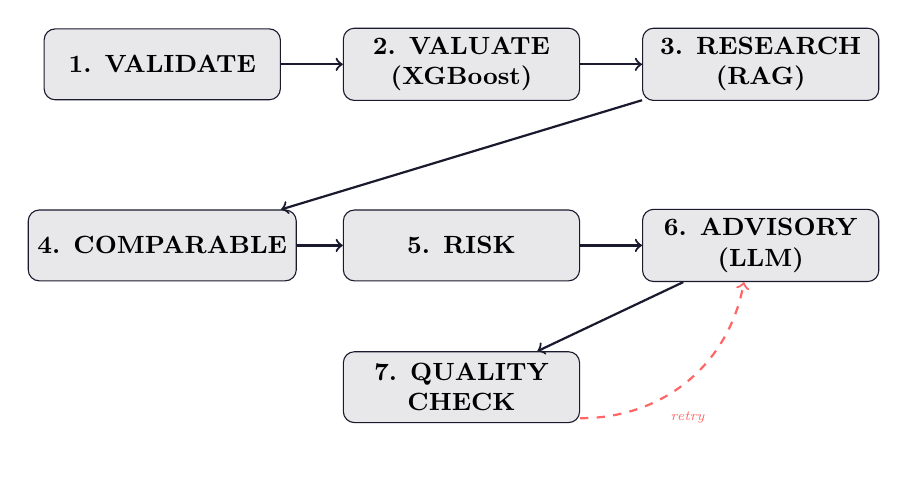
\begin{tikzpicture}[
    node distance=1.8cm,
    every node/.style={rectangle, draw=darkbg, fill=darkbg!10, rounded corners=4pt, minimum width=3cm, minimum height=0.9cm, font=\small\bfseries, align=center},
    arrow/.style={->, thick, color=darkbg}
]
\node (v) {1. VALIDATE};
\node (p) [right of=v, xshift=2cm] {2. VALUATE\\(XGBoost)};
\node (r) [right of=p, xshift=2cm] {3. RESEARCH\\(RAG)};
\node (c) [below of=v, yshift=-0.5cm] {4. COMPARABLE};
\node (k) [right of=c, xshift=2cm] {5. RISK};
\node (a) [right of=k, xshift=2cm] {6. ADVISORY\\(LLM)};
\node (q) [below of=k] {7. QUALITY\\CHECK};

\draw[arrow] (v) -- (p);
\draw[arrow] (p) -- (r);
\draw[arrow] (r) -- (c);
\draw[arrow] (c) -- (k);
\draw[arrow] (k) -- (a);
\draw[arrow] (a) -- (q);
\draw[arrow, dashed, color=red!60] (q) to[bend right=40] node[midway, below, font=\tiny\itshape, draw=none, fill=none] {retry} (a);
\end{tikzpicture}
\caption{LangGraph 7-Node Pipeline with Conditional Retry}
\end{figure}

\subsection{Technology Stack}
\begin{table}[H]\centering
\caption{Technology Stack}
\begin{tabular}{@{}ll@{}}
\toprule
\textbf{Layer} & \textbf{Technology} \\
\midrule
Agent Framework & LangGraph (StateGraph + conditional edges) \\
LLM Provider & Groq \texttt{llama-3.3-70b-versatile} (free tier) \\
ML Model & XGBoost (gradient boosted trees) \\
Vector Store & ChromaDB + HuggingFace \texttt{all-MiniLM-L6-v2} \\
State Management & Python \texttt{TypedDict} with \texttt{Annotated} operators \\
Web UI & Streamlit (glassmorphism dark theme) \\
PDF Export & ReportLab \\
Knowledge Sources & JLL, Knight Frank, RERA Act, curated markdowns \\
\bottomrule
\end{tabular}
\end{table}

%═══════════════════════════════════════════
\section{Agentic AI Pipeline — Detailed Design}
%═══════════════════════════════════════════

\subsection{State Management}
The pipeline uses a \texttt{TypedDict} with 12 typed fields:

\begin{lstlisting}[language=Python, basicstyle=\ttfamily\small, frame=single, breaklines=true]
class AgentState(TypedDict):
    property_input: dict
    user_preferences: dict
    predicted_price: float
    confidence_score: float
    market_context: Annotated[List[str], operator.add]
    rera_context: str
    comparable_properties: list
    risk_assessment: dict
    market_sentiment: dict
    final_advisory: str
    report_sections: dict
    agent_trace: Annotated[List[str], operator.add]
\end{lstlisting}

The \texttt{Annotated[List[str], operator.add]} pattern ensures market context and agent traces are \textbf{appended} across nodes rather than overwritten.

\subsection{Node Descriptions}
\begin{enumerate}
    \item \textbf{Validate Node} — Normalizes input, fills defaults, validates required fields. Pure Python logic.
    \item \textbf{Valuate Node} — Runs XGBoost prediction on 10 features, computes confidence score based on city tier and price-per-sqft typicality.
    \item \textbf{Research Node} — Dual RAG retrieval: \texttt{market\_researcher} (general trends) and \texttt{rera\_researcher} (legal). Top-5 similarity search with source attribution.
    \item \textbf{Comparable Node} — Generates 5--6 property variations ($\pm$BHK, $\pm$20\% size, furnishing change) by re-running the ML model with modified features.
    \item \textbf{Risk Node} — 4-factor risk matrix: interest rate sensitivity, market cycle position, valuation benchmark, liquidity risk. Includes EMI calculations at 4 rates.
    \item \textbf{Advisory Node} — LLM synthesizes all data into a 5-section structured report using anti-hallucination prompting.
    \item \textbf{Quality Check Node} — Validates all 5 sections exist via regex. If incomplete, triggers a conditional retry (max 1).
\end{enumerate}

%═══════════════════════════════════════════
\section{RAG Implementation}
%═══════════════════════════════════════════

\subsection{Knowledge Base}
\begin{table}[H]\centering
\caption{Knowledge Base Sources (656 total chunks)}
\begin{tabular}{@{}lll@{}}
\toprule
\textbf{Source} & \textbf{Type} & \textbf{Content} \\
\midrule
RERA Act.pdf & Legal & Full RERA legislation \\
JLL Q4 2023.pdf & Market & Quarterly residential update \\
Knight Frank H1 2024.pdf & Market & Residential \& office analysis \\
Affordable Housing 2025.pdf & Policy & India housing report \\
india\_market\_overview.md & Curated & City-wise prices for 8 cities \\
rera\_compliance\_guide.md & Curated & RERA provisions \& penalties \\
investment\_guidelines.md & Curated & Buy/Hold/Sell indicators \\
\bottomrule
\end{tabular}
\end{table}

\subsection{Retrieval Pipeline}
\begin{itemize}[noitemsep]
    \item \textbf{Chunking}: \texttt{RecursiveCharacterTextSplitter} (1000 chars, 150 overlap)
    \item \textbf{Embeddings}: HuggingFace \texttt{all-MiniLM-L6-v2} (384-dim vectors)
    \item \textbf{Vector Store}: ChromaDB with persistent storage
    \item \textbf{Retrieval}: Top-5 similarity search per query
    \item \textbf{Source Attribution}: Every chunk tagged with source filename
    \item \textbf{Lazy Loading}: Singleton pattern prevents macOS segfault on import
\end{itemize}

%═══════════════════════════════════════════
\section{Anti-Hallucination \& Responsible AI}
%═══════════════════════════════════════════

\begin{table}[H]\centering
\caption{Anti-Hallucination Strategies}
\begin{tabular}{@{}lp{8cm}@{}}
\toprule
\textbf{Strategy} & \textbf{Implementation} \\
\midrule
RAG-grounded citations & LLM instructed to cite ONLY from provided context \\
Source attribution & Every RAG chunk tagged with source filename \\
Confidence scoring & ML predictions include a heuristic confidence metric \\
Structured enforcement & Quality Check validates all 5 sections exist \\
Retry loop & Incomplete reports trigger automatic re-generation \\
Explicit uncertainty & LLM states ``Data not available'' instead of guessing \\
Mandatory disclaimer & Every report includes legal/financial disclaimer \\
\bottomrule
\end{tabular}
\end{table}

%═══════════════════════════════════════════
\section{User Interface}
%═══════════════════════════════════════════

The Streamlit UI features:
\begin{itemize}[noitemsep]
    \item \textbf{7 Agent Deployment Cards} — live status: Deployed $\rightarrow$ Working $\rightarrow$ Complete
    \item \textbf{Glassmorphism dark theme} with neon green (\texttt{\#00ffcc}) accents
    \item \textbf{5 Metric Cards} — Price, City, Confidence, Sentiment, Risk
    \item \textbf{Tabbed report display} — 5-section structured advisory
    \item \textbf{Comparable properties table} — interactive DataFrame
    \item \textbf{EMI scenarios} — 4 interest rate comparisons
    \item \textbf{PDF download} — one-click branded export
    \item \textbf{Agent trace panel} — full reasoning log
\end{itemize}

%═══════════════════════════════════════════
\section{Model Performance \& Evaluation}
%═══════════════════════════════════════════

\subsection{Test Results}
All 32 tests pass across 8 test suites:

\begin{table}[H]\centering
\caption{Test Results Summary}
\begin{tabular}{@{}lcc@{}}
\toprule
\textbf{Test Suite} & \textbf{Tests} & \textbf{Status} \\
\midrule
ML Model (prediction, confidence, multi-city) & 5 & \textcolor{primary}{PASS} \\
RAG Retrieval (market, RERA, sources, cities) & 7 & \textcolor{primary}{PASS} \\
Comparable Analyzer (generation, structure) & 3 & \textcolor{primary}{PASS} \\
Risk Simulator (factors, EMI, sentiment) & 5 & \textcolor{primary}{PASS} \\
Market Sentiment (bullish, bearish, infra) & 4 & \textcolor{primary}{PASS} \\
PDF Report Generator (full, minimal) & 2 & \textcolor{primary}{PASS} \\
Node Transitions (5 nodes individually) & 5 & \textcolor{primary}{PASS} \\
Full E2E Pipeline (all 7 nodes + LLM) & 1 & \textcolor{primary}{PASS} \\
\midrule
\textbf{Total} & \textbf{32} & \textbf{ALL PASS} \\
\bottomrule
\end{tabular}
\end{table}

\subsection{Key ML Results}
\begin{itemize}[noitemsep]
    \item Mumbai 3BHK Apartment (1800 sqft): \textbf{Rs 12.95 Lakhs}
    \item Tier-1 city confidence: \textbf{0.75}, Tier-2: \textbf{0.60}
    \item Size-price relationship validated: 800 sqft (Rs 9.33L) $\rightarrow$ 2000 sqft (Rs 12.96L)
    \item Comparable generation: 5 variants with correct price differentials
\end{itemize}

%═══════════════════════════════════════════
\section{Deployment}
%═══════════════════════════════════════════

\begin{lstlisting}[basicstyle=\ttfamily\small, frame=single, breaklines=true]
# Install dependencies
pip install -r requirements.txt

# Build knowledge base (first time)
python -m src.tools.ingest

# Run application
streamlit run streamlit_app.py

# Run all tests
python tests/test_ml.py
python tests/test_rag.py
python tests/test_comparables.py
python tests/test_risk.py
python tests/test_sentiment.py
python tests/test_pdf.py
python tests/test_nodes.py
python tests/test_full_agent.py
\end{lstlisting}

\textbf{Environment}: Set \texttt{GROQ\_API\_KEY} in \texttt{.env} file (free key from \url{https://console.groq.com/keys}).

%═══════════════════════════════════════════
\section{Conclusion}
%═══════════════════════════════════════════

Estate Agent AI demonstrates a production-grade agentic AI system that autonomously reasons about property value, retrieves market trends via RAG, and generates structured investment recommendations. The 7-node LangGraph pipeline with conditional retry logic, multi-source knowledge base (656 chunks), and anti-hallucination strategies ensure reliable, grounded advisory output. All 32 automated tests pass, and the system is deployment-ready on Streamlit Community Cloud.

\subsection{Future Work}
\begin{itemize}[noitemsep]
    \item LangSmith integration for agent observability and tracing
    \item Expanded knowledge base with quarterly report auto-ingestion
    \item Multi-language advisory support (Hindi, Marathi, Tamil)
    \item Real-time web scraping for live property listings
\end{itemize}

\end{document}
